\chapter{تخصیص برش شبکه به صورت دینامیکی}
\section{مقدمه}
در این فصل هدف تخصیص برش شبکه به صورت می‌باشد. در فصل قبلی مدل سیستم به طور کامل نوشته شده است و در حالت آفلاین حل گردیده است، در این فصل پارامترها مورد نیاز را نسبت به فصل قبلی کمتر کرده و با استفاده از روش دینامیکی در هر لحظه از زمان به حل سیستم می‌پردازیم. برای حل این سیستم از روش یادگیری تقویتی عمیق استفاده می‌کنیم.
در بخش اول صورت مسئله‌ی بخش رادیویی نوشته می‌شود. سپس به صورت مسئله و مدل سیستم بخش هسته می‌پردازیم و در نهایت روش حل هر دو مسئله و نتایج عددی آن بیان می‌شود.
\section{ مدل سیستم و صورت مسئله‌ی اول}
در این بخش هدف برش شبکه در بخش رادیویی سیستم می‌باشد. دراینجا، مسئله‌ی اول فصل قبلی ساده شده و به روش دینامیکی حل می‌شود.   
همانند سیستم فصل قبل، فرض می کنیم $S$ برش شبکه داریم که قرار است $V$ سرویس مختلف که شامل کاربرانی است که از سرویس خاص استفاده می‌نمایند را سرویس دهی نماید.
هر سرویس 
$v\in \{1,2,...,V \} $
شامل تعدادی کاربر تک آنتنه می باشند که سرویس خاصی را درخواست می‌نماید.
هر برش شبکه
$s\in \{1,2,...,S \} $
 شامل تعدادی
 PRB
  RU،
   BBU، 
   و
    VNF 
 می‌باشد.
در این بخش سعی برا‌ین است که در ابتدا مسئله را به ساده‌ترین حالت ممکن حل نماییم. فرض می‌کنیم سه مدل سرویس مختلف داریم که سرویسهای دسته‌ی اول نیازمند تاخیر خاص و سرویسهای دسته‌ی دوم نیازمند داشتن تاخیر کم هستند و سرویس سوم نیازمند داشتن هر دو حالت تاخیر کم و نرخ زیاد است.
در بخش اول این مسئله، هدف بیشینه‌سازی تعدای سرویسهای پذیرفته شده می‌باشد. در اینجا فرض براین است که تعداد برشهاس شبکه محدود می‌باشد. فرض می‌کنیم هر سرویس $v$ دارای اولویت $p_v$ می‌باشد. 
همچنین فرض براین است که هر سرویس شامل ماکسیمم $U_v$ کاربر است و به طور میانگین کاربران آن نیازمند داشتن نرخ بیشتر از $R_v$ و تاخیر کمتر از $D_v$ هستند. درصورتی که کاربری از دسته‌ی اول باشد 
$D_v =  M$ 
که $M$ برای تاخیر یک عدد بزرگ می‌باشد.
و در صورتی که سرویس از دسته‌ی دوم باشد 
$R_v = N $
که $N$ یک عدد کوچک برای نرخ می‌باشد.
صورت مسئله به صورت \eqref{eqmain} می‌باشد.
در اینجا برای سادگی فرض براین است که هر سرویس به ماکسیمم یک برش شبکه متصل می‌گردد. در اینجا هدف حل مسئله در هر اسلات زمانی t می‌باشد.
 هدف در اینجا بیشینه سازی تعداد سرویسهای پذیرفته شده توسط برشهای شبکه می‌باشد به صورتی که شرط تاخیر و نرخ سرویس را ضمانت کنند.
\begin{subequations}
	\begin{alignat}{4}
		\max\limits_{\boldsymbol{a}(t) }   \quad &   \sum_{s=1}^{S(t)}\sum_{v=1}^{V(t)} p_v a_{v,s}(t)\\
		\text{\lr{subject to}} \quad & \textstyle \sum_{s=1}^{S(t)} D_s(t) a_{v,s} \leq D_v(t)  \forall v, \\
		&\textstyle   \sum_{s=1}^{S(t)} R_s(t) a_{v,s}(t) \geq R_v(t)  \forall v \label{eqmain}
	\end{alignat}
	\label{constraints2}
\end{subequations}
 برای اینکه معادله‌ی 
 \eqref{eqmain}
 را به فرم مسئله‌ی کوله‌پشتی دربیاوریم، از آنجایی که فرض کردیم هر سرویس به ماکسیمم یک برش شبکه متصل می‌شود، می‌توان معادله بدین صورت نوشت:
 \begin{subequations}
 	\begin{alignat}{4}
		\max\limits_{\boldsymbol{a}(t) }   \quad &   \sum_{s=1}^{S(t)}\sum_{v=1}^{V(t)} p_v a_{v,s}(t)\\
		\text{\lr{subject to}} \quad & \textstyle \sum_{s=1}^{S(t)} D_s(t) a_{v,s} \leq D_v(t)  \forall v, \\
 		&\textstyle   \sum_{s=1}^{S(t)} \frac{1}{R_s(t)} a_{v,s}(t) \leq \frac{1}{R_v(t)}  \forall v \label{eqmain1}
 	\end{alignat}
 	\label{constraints2}
 \end{subequations}
که در اینجا، معادله‌ی \eqref{eqmain1}
یک معادله‌ی کوله‌پشتی دو بعدی می‌باشد.
برای حل این مسئله، از روش یادگیری تقویتی استفاده می‌شود.
\section{ مدل سیستم و صورت مسئله‌ی دوم}
در این بخش سعی شده، مسئله‌ی دوم فصل قبل به صورت ساده شده با روش دینامیکی حل شود. عنوان این مسئله، جاگزاری VNFها برروی مراکز داده می‌باشد.
فرض براین است که $S$ برش شبکه داریم که هر برش شبکه s
$s\in \{1,2,...,S \} $
می‌باشد. هر برش شبکه شامل تعدادی VNF است که
هر \lr{VNF}
نیازمند منابع فیزیکی است که شامل حافظه، نگهدارنده و پردازشگر می باشد.
فرض کنید برای سادگی مسئله برای هر VNF به مقدار کافی حافظه و نگهددارنده در مراکز داده داریم و تنها منبع مورد نیاز برای $f$ امین \lr{VNF} در برش $s$ ام مقدار پردازنده است که به صورت $\bar{\Omega}_{s}^f$ می باشد 
%\begin{equation}
%	\bar{\Omega}_{s}^f = \{\Omega_{M,{s}}^f, \Omega_{S,{s}}^f, \Omega_{C,{s}}^f \},
%\end{equation}
که در اینجا 
$\bar{\Omega}_{s}^f\in \mathbb{C}^{1}$
و
%$\Omega_{M,{s}}^f, \Omega_{S,{s}}^f, \Omega_{C,{s}}^f$
%به ترتیب نشان دهنده ی مقدار حافظه، نگهدارنده و پردازشگر می باشد.
%همچنین مقدار کل حافظه، نگهدارنده و پردازشگر برای همه \lr{VNF} ها در یک برش به این صورت تعریف می شود
\begin{equation}
	\textstyle \bar{\Omega}_{s}^{tot} = \sum_{f=1}^{M_{s}}\bar{\Omega}_{s}^f %\;\; \mathfrak{z} \in \{M, S, C\}.
\end{equation}
همچنین $D_c$ مرکز داده برای سرویس دهی به \lr{VNF} ها می باشد. هر مرکز داده شامل تعدادی سرور برای سرویس دهی است.$M_s$ تعداد کل VNFها در sامین برش شبکه است.
مقدار پردازشگر 
%$\tau_{M_{j}}, \tau_{S_{j}}$
%و
$\tau_{j} $
برای 
$j$
امین مرکز داده  می‌باشد.
%\begin{equation*}
%	\tau_j = \{\tau_{M_{j}}, \tau_{S_{j}}, \tau_{C_{j}} \},
%\end{equation*}
در این مدل سیستم، 
تخصیص منابع فیزیکی به \lr{VNF} ها در نظر گرفته شده است. 
در اینجا فرض بر این است که $y_{s,d}$ متغیر صفر و یکی است که نشان میدهد مرکز داده ی $d$ ام به $s$ امین برش متصل است یا نه. 
همانند فصل قبل، 
فرض کنید توان مصرفی پردازش باند پایه در هر مرکز داده ی $d$ که به \lr{VNF} های یک برش $s$ متصل می باشد در هر زمان t با   
$\phi_{s,d}(t)$
نشان داده شده است.
بنابراین می توان توان کل سیستم را برای کلیه مرکز داده های فعال که به برش متصل هستند ،بدین صورت نشان داد
\begin{equation*}
	\textstyle \phi_{tot}(t) = \sum_{s=1}^{S}\sum_{d=1}^{D_c}y_{s,d}\phi_{s,d}(t).
\end{equation*}
همچنین ، یک تابع هزینه برای قرار
همچنین فرض کنید در هر زمان قرار دادن هر مجموعه‌ی جدید VNFهای برش شبکه s برروی مرکز داده d مقدار انرژی اضافی را بدین صورت به سیستم اعمال کنند.
\begin{equation*}
	\textstyle \phi_{diff}(t) = \sum_{s=1}^{S}\sum_{d=1}^{D_c}[y_{s,d}(t)-y_{s,d}(t-1)]^+\phi_{s,d}^{new}(t).
\end{equation*}
%%
تابع هزینه‌ی قرارگیری VNFها برروی DCها بدین صورت است
\begin{equation}\label{eqpsi}
	\textstyle  \psi_{tot}(t) = \phi_{tot}(t) + \phi_{diff}(t)
\end{equation}
در اینجا هدف کمینه کردن مقدار انرژی کل در هر زمان، با فرض اینکه مجموع VNFهای برشهای تخصیص یافته به هر مرکز داده مقدار کافی پردازنده داشته باشند. در اینجا فرض براین است که برشهای شبکه که قبلا به سرویسها اختصاص داده شده، می‌بایست در مرکز داده قرار داده شوند و تعداد مراکز داده به اندازه‌ی کافی زیاد هستند، هدف کمینه کردن انرژی است به صورتی که کمترین تعداد مرکز داده‌ها استفاده شوند.
\begin{subequations}
	\begin{alignat}{4}
		\min\limits_{\boldsymbol{y} }   \quad &   \psi_{tot}(\boldsymbol{Y})(t)\\
		\text{s. t.} \quad & \textstyle \sum_{d=1}^{D_c} y_{s,d}(t) \geq 1 \quad \forall s, \\
		&\textstyle  \sum_{s=1}^{S} y_{s,d}(t) \bar{\Omega}_{s}^{tot}  \leq   \tau_{d} \quad  \forall d, \forall ;  \label{eqomega}
	\end{alignat}
\end{subequations}
این مسئله به فرم مسئله‌ی بسته‌بندی جعبه قابل بیان است.
\section{حل مسئله به‌روش یادگیری تقویتی}
دراینجا از روش یادگیری تقویتی در حل دو مسئله‌ی بالا استفاده می‌نماییم.
در روش یادگیری تقویتی، یک عامل سعی می‌کند رفتار بهینه را در یک محیط مشخص پیدا کند. این پروسه‌ی تعاملی، به صورت پروسه‌ی تصمیم‌گیری مارکوف مدل می‌شود که شامل $(S,A,R,P,\gamma)$  می باشد.
S
نشان‌دهنده‌ی ماتریس فضای حالت و A بردار رفتار می‌باشد. R نیز پاداش عمل است. 
$P(.|s,a)$
احتمال انتقال و
 $\gamma \in (0,1]$
 فاکتور تخفیف می‌باشد.
 سیاست 
$\Pi(.|s)$
نگاشتی از حالت به توزیع اعمال می‌باشد.
تابع مقدار-حالت برای حالت s تحت سیاست $\Pi(.|s)$ را با  
$V^{\Pi}(s)$
نشان می‌دهند که مقدار بازده مورد انتظار در حالت s تحت سیاست $\Pi(.|s)$
می‌باشد. مقدار ارزش انجام عمل a در حالت s تحت سیاست $\Pi(.|s)$ 
را با
 $Q^{\Pi}(s,a)$
 نمایش می‌دهیم.
 که روابط زیر را براین اساس داریم.
 \begin{equation}
	V^{\Pi}(s) = \mathbb{E}_{\Pi,P}[\sum_{t=0}^{\infty}\gamma^tR_t|S_0=s]
 \end{equation}
و تابع ارزش عمل بدین صورت است

 \begin{equation}
	Q^{\Pi}(s,a) = \mathbb{E}_{\Pi,P}[\sum_{t=0}^{\infty}\gamma^tR_t|S_0=s,A_0=a]
\end{equation}
  که در اینجا 
  $\mathbb{E}$
  میانگین می‌گیرد.
  باتوجه به رابطه‌ی بلمن، داریم:
 \begin{equation}
	V^{\Pi}(s) = \mathbb{E}_{\Pi,P}[R+\gamma V^{\Pi}(s')]
\end{equation}  
  و داریم:
   \begin{equation}
  	Q^{\Pi}(s,a) = \mathbb{E}_{\Pi,P}[R+\gamma Q^{\Pi}(s',a')]
  \end{equation}  
که دراینجا $s'$
و $a'$
قابل اتخاذ از 
$P(.|s,a)$
و سیاست
$\Pi(.|s')$
هستند.
هدف یادگیری تقویتی، بدست‌آوردن سیاست بهیته می‌باشد به صورتی که 
$Q^{\Pi}(s,a)$
بیشینه شود.
مقدار بهینه‌ی تابع ارزش عمل در رابطه‌ی بلمن بدین صورت است

\begin{equation}
	Q^{*}(s,a) = \mathbb{E}_{\Pi^*,P}[R+\gamma Q^{*}(s',a')]
\end{equation} 
همچنین در صورت تعریف اپراتور $T^*$ بلمن داریم
\begin{equation}
	T^{*}Q(s,a) = \mathbb{E}_{\Pi^*,P}[R+\gamma Q(s',a')]
\end{equation} 
که به صورت تکراری اعمال این اپراتور 
$Q_{t+1}(s,a) \leftarrow T^{*}Q(s,a) $
منجر به همگرا شدن 
$Q_{t}(s,a) \rightarrow Q^*(s,a)$
 و
 $t \rightarrow \infty $
می‌شود
\cite{montague1999reinforcement,gan1}.
در ابعاد بالاتر، بهتر است از تابع تقریبی استفاده
شود. فرض کنید 
$Q_{\theta}(s,a)$
تابع تقریب با پارامتر $\theta$
می‌باشد که تقریبی از جدول مقدار عمل با (s,a)
می‌باشد. هدف این بهینه‌سازی، بدست‌آوردن $\theta$
است به طوری که 
$Q_{\theta}(s,a) \approxeq Q^{*}(s,a)$
و مقدار بهینه، به طور تکراری با اعمال اپراتور $T^*$
بدست می‌آید. 
مقدار بهینه‌ی 
$\theta$
قابل دستیابی با استفاده از مینیمم کردم خطای تفاوت زمانی (TD-error)
برروی (s,a,r,s') می‌باشد که به طور رندم انتخاب می‌شوند.
\begin{equation}
\zeta^2 = [r + \gamma \max_{a' \in A}{Q_{\theta}(s',a')}-Q_{\theta}(s,a)]^2
\end{equation}
روشهای مخنلفی برای دستیابی به مینیمم خطا هست که ما در ادامه‌ی کار از روش Q-learnng استفاده می‌کنیم.
در روش Q-learning در هر بروزرسانی تابع Q داریم:
\begin{equation}
	Q(s_{t+1},a_{t+1}) = Q(s_t,a_t)+\alpha[ r_{t+1} + \gamma \max_{a \in A}{Q(s_{t+1},a)}-Q(s_t,a_t)]
\end{equation}
که دراینجا، $\alpha$
نرخ یادگیری می‌باشد.
\subsection{نتایج عددی مسئله‌ی اول}
در این بخش، برای مسئله‌ی اول حالت، عامل و پاداش را تعیین می‌نماییم و سپس نتایج عملی را نشان می‌دهیم.
در این مسئله، عامل، orchestrator است که وظیفه‌ی مدیریت شبکه را برعهده دارد.
همچنین، حالت در هر بازه‌ی زمانی برشهایی از شبکه است که به سرویسها متصل شده و همچنین مقدار منبع باقی ماده در هر برش می‌باشد. 
پاداش طوری تعیین شده که بیشترین تعداد سرویسها پذیرفته شود به طوریکه شرط تاخیر و نرخ برآورده گردد.
برای حل این مسئله به روش دینامیکی، دو مدل سرویس در نظر گرفتیم و شرط تاخیر در این دو مدل سرویس اعمال نشده‌است.
در این بخش، به دلیل کم بودن تعداد حالتها، از روش Q-Learning استفاده کرده و برای جدول Q نیاز به استفاده از روش یادگیری عمیق نیست.
در مدل اول سرویس نیازمند نرخ $10MHz$ و مدل دوم سرویس نیازمند نرخ $20MHz$
می‌باشد. فرض می‌کنیم نرخ ورود سرویس در هر ابتدای بازه‌ی زمانی عدد رندم با توزیع پواسون می‌باشد. نرخ خروج سرویس نیز از توزیع نرمال پیروی می‌کند. در اینجا فرض می کنیم از  سرویس اول ماکسیمم در هر لحظه 8 سرویس و از سرویس دوم 4 تا سرویس درخواست می‌دهد. 2 برش شبکه با نرخ $40MHz$ نیز وجود دارد. 
در شکل \ref{fig:dynamicEpoch}
نسبت تعداد سرویسهای پذیرفته شده به نسبت تعداد سرویسهای پذیرفته شده در حالت بهینه براساس زمان طی شده داده می‌شود. بعد از حدود 900 تکرار مسئله، تقریبا خروجی با خروجی بهینه یکی می‌شود و مقدار پذیرفته شده با مقدار بهینه تقریبا یکی می‌شود. بعد از حدود 4000 تکرار، تقریبا احتمال انتخاب عمل رندم صفر می‌شود و صرفا با استفاده از تابع Q، عمل انتخاب می‌شود.
در اینجا از روش 
$\epsilon-greedy$
برای حل استفاده شده است.

\begin{figure}%[H]
	\centering
	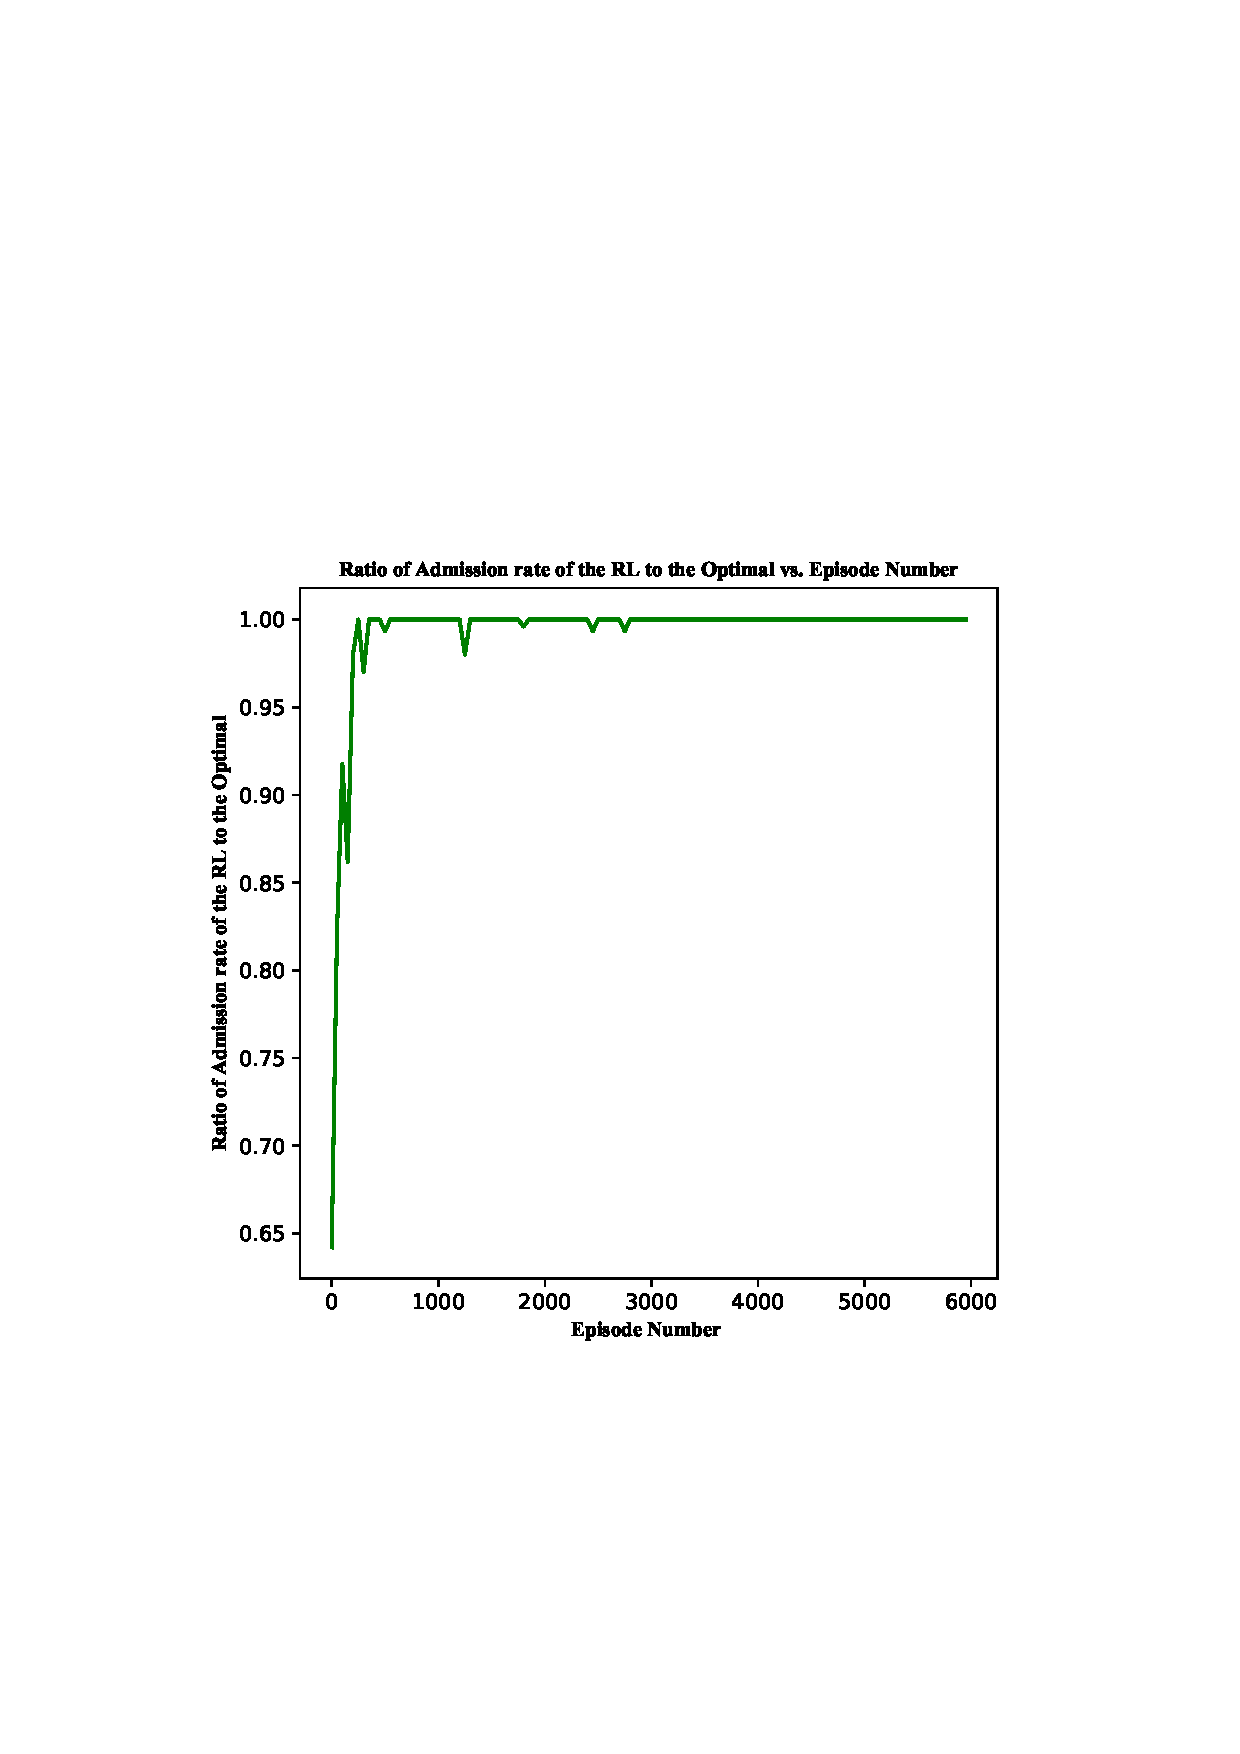
\includegraphics[scale = 0.6]{./fig/dynamicEpoch_0} %[width=\linewidth] 
	\caption{  نسبت تعداد سرویسهای پذیرفته شده با استفاده از روش یادگیری تقویتی عمیق به نسبت تعداد سرویسهای پذیرفته شده در حالت بهینه براساس زمان طی شده}
	\label{fig:dynamicEpoch}
\end{figure}
در شکل \ref{fig:dynamicEpoch1}
با افزایش تعداد برشها و بیشینه تعداد درخواستها در هر زمان، بعد از 1000 تکرار سناریو جواب به حالت بهینه نزیک شده ولی هیچ موقع با مقدار بهینه برابری نمی‌کند. در اینجا، تعداد درخواستهای سرویس اول 10 تا و سرویس دوم 5 تا می‌باشد. همچنین نرخ خروج عدد رندم یکنواخت است. 
\begin{figure}%[H]
	\centering
	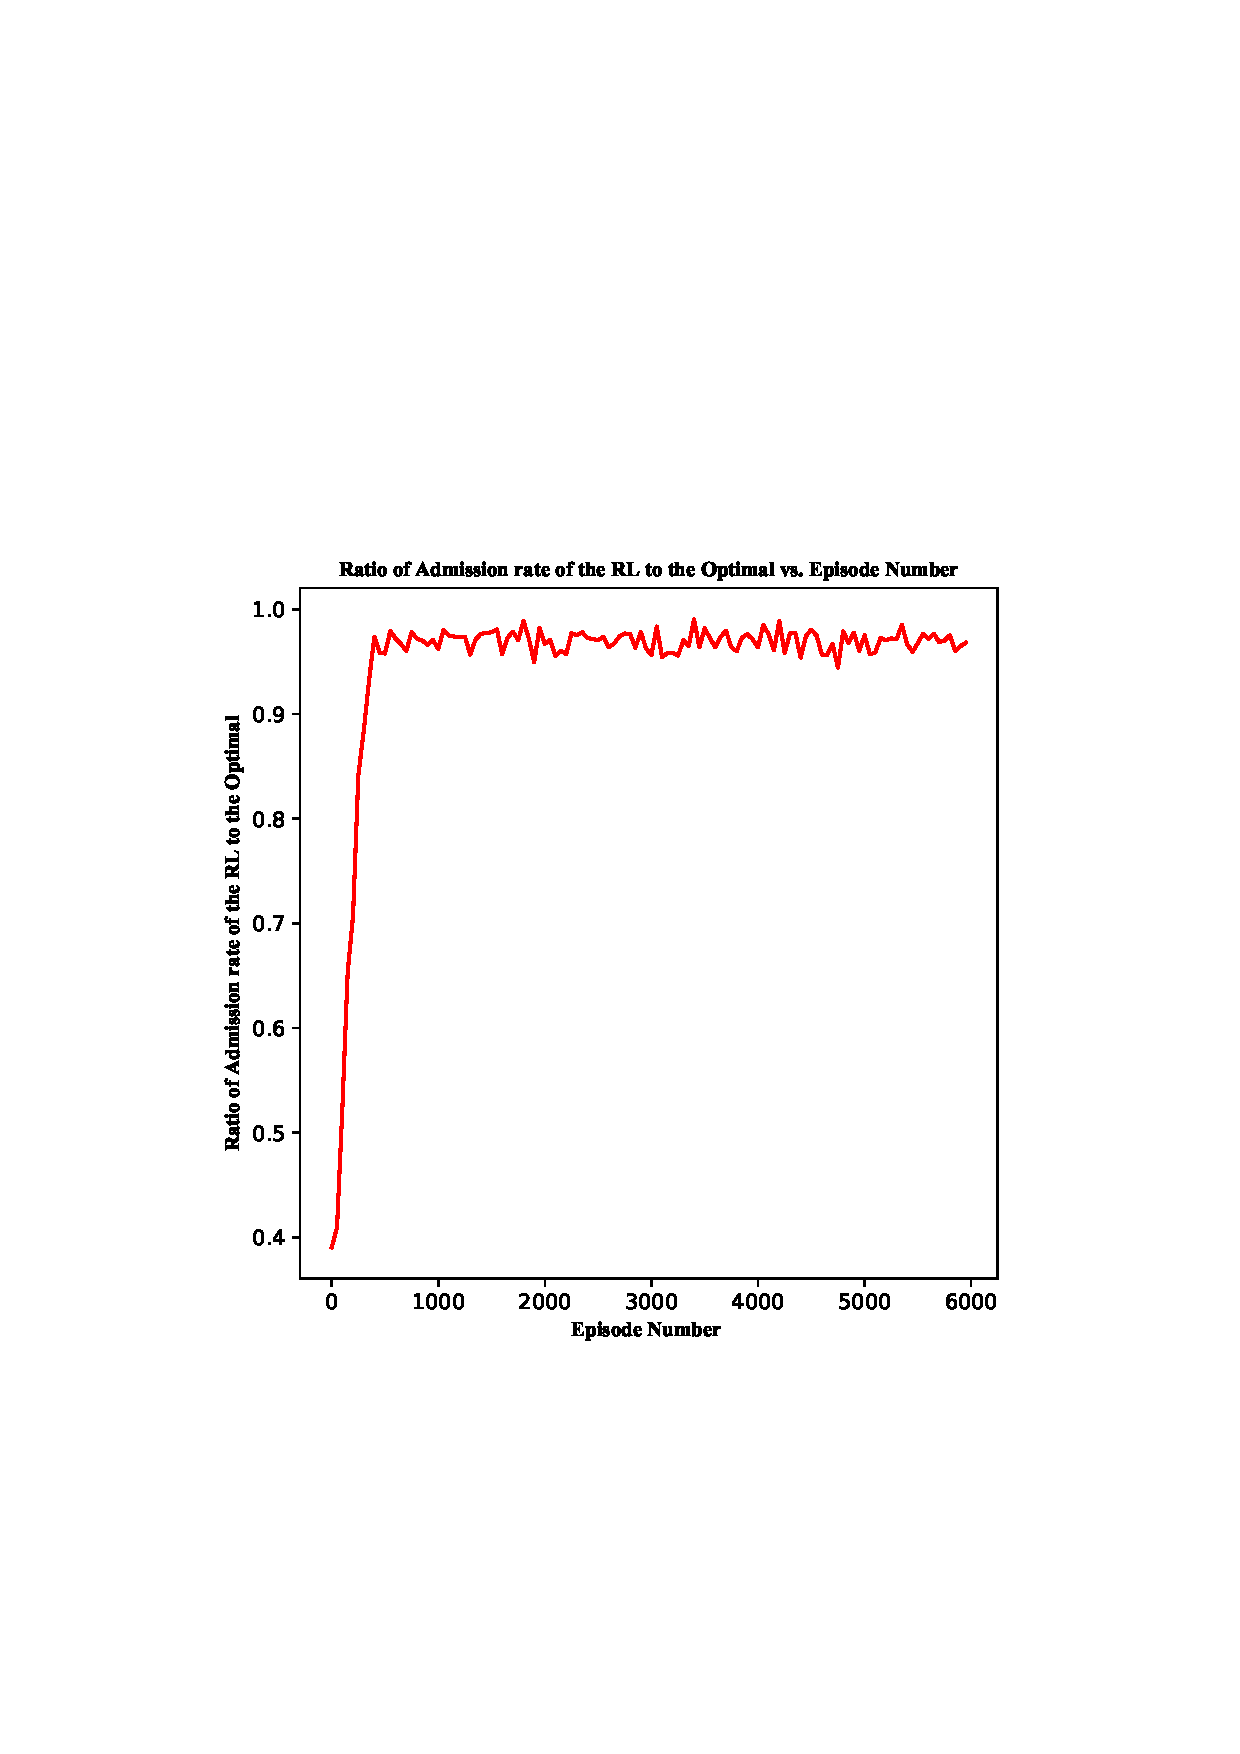
\includegraphics[scale = 0.6]{./fig/dynamicEpoch1_0} %[width=\linewidth] 
	\caption{  نسبت تعداد سرویسهای پذیرفته شده روش استفاده شده به نسبت تعداد سرویسهای پذیرفته شده در حالت بهینه براساس زمان طی شده با افزایش تعداد ماکسیمم درخواستها و تعداد برشهای شبکه}
	\label{fig:dynamicEpoch1}
\end{figure}
\subsection{نتایج عددی مسئله‌ی دوم} 
در این بخش، برای مسئله‌ی دوم حالت، عامل و پاداش را تعیین می‌نماییم و سپس نتایج عملی را نشان می‌دهیم.
در این مسئله، عامل، orchestrator است که وظیفه‌ی مدیریت شبکه را برعهده دارد.
همچنین، حالت در هر بازه‌ی زمانی برشهایی از شبکه است که به مراکزداده متصل شده و اینکه کدام برش به کدام مرکز داده متصل است.
پاداش طوری تعیین شده که کمترین تعداد مراکز داده استفاده گردد و هر لحظه کمترین تعداد مرکز داده‌ی خاموش، روشن شود.
\section{نتیجه‌گیری}
در این فصل، دو مسئله‌ی فصل قبلی به صورت ساده شده نوشته شد و مسئله‌ی اول در بخش رادیویی از جنس کوله‌پشتی و مسئله‌ی دوم در بخش هسته از نوع 
بسته‌بندی جعبه می‌باشد. این دو مسئله به صورت دینامیکی در هر لحظه از زمان حل شده‌اند. برای حل این دو مسئله از روش یادگیری تقویتی عمیق استفاده شده و حالتها و اعمال بیان برای یک عامل در این مسئله بیان گرده است.
نتایج عملی آن نیز رسم گردید.

  